% \documentclass[aspectratio=169,notes]{beamer}
\documentclass[aspectratio=169]{beamer}
\usetheme[faculty=phil]{fibeamer}
\usepackage{polyglossia}
\setmainlanguage{english} %% main locale instead of `english`, you
%% can typeset the presentation in either Czech or Slovak,
%% respectively.
\setotherlanguages{russian} %% The additional keys allow
%%
%%   \begin{otherlanguage}{czech}   ... \end{otherlanguage}
%%   \begin{otherlanguage}{slovak}  ... \end{otherlanguage}
%%
%% These macros specify information about the presentation
\title[MaM]{Mechanics and Machines, CAE STR 1} %% that will be typeset on the
\subtitle{Stress Analysis
\\ \  \\ \ 
    } %% title page.
\author{Oleg Bulichev}
%% These additional packages are used within the document:
\usepackage{ragged2e}  % `\justifying` text
\usepackage{booktabs}  % Tables
\usepackage{tabularx}
\usepackage{tikz}      % Diagrams
\usetikzlibrary{calc, shapes, backgrounds}
\usepackage{amsmath, amssymb}
\usepackage{url}       % `\url`s
\usepackage{listings}  % Code listings
% \usepackage{subfigure}
\usepackage{floatrow}
\usepackage{subcaption}
\usepackage{mathtools}
\usepackage{todonotes}
\usepackage{fontspec}
\usepackage{multicol}
\usepackage{pdfpages}
\usepackage{wrapfig}
\usepackage{animate}
\usepackage{booktabs}
\usepackage{multirow}
% \usepackage{graphicx}
\usepackage{colortbl}

\graphicspath{{resources/}}
\frenchspacing

\setbeamertemplate{caption}[numbered]
\usetikzlibrary{graphs}

% \usepackage[backend=biber,style=ieee,autocite=footnote]{biblatex}
% \addbibresource{biblio.bib}
% \DefineBibliographyStrings{english}{%
%   bibliography = {References},}

\newcommand{\oleg}[2][] {\todo[color=red, #1] {OLEG:\\ #2}}
\newcommand{\fbckg}[1]{\usebackgroundtemplate{\includegraphics[width=\paperwidth]{#1}}}%frame background

\usepackage[framemethod=TikZ]{mdframed}
\newcommand{\dbox}[1]{
\begin{mdframed}[roundcorner=3pt, backgroundcolor=yellow, linewidth=0]
\vspace{1mm}
{#1}
\vspace{1mm}
\end{mdframed}
}

\begin{document}
\setlength{\abovedisplayskip}{0pt}
\setlength{\belowdisplayskip}{0pt}
\setlength{\abovedisplayshortskip}{0pt}
\setlength{\belowdisplayshortskip}{0pt}

\fbckg{fibeamer/figs/title_page.png}
\frame[c]{\setcounter{framenumber}{0}
    \usebeamerfont{title}%
    \usebeamercolor[fg]{title}%
    \begin{minipage}[b][6.5\baselineskip][b]{\textwidth}%
        \textcolor{black}{\raggedright\inserttitle}
    \end{minipage}
    % \vskip-1.5\baselineskip

    \usebeamerfont{subtitle}%
    \usebeamercolor[fg]{framesubtitle}%
    \begin{minipage}[b][3\baselineskip][b]{\textwidth}
        \raggedright%
        \insertsubtitle%
    \end{minipage}
    \vskip.25\baselineskip
}
%   \frame[c]{\maketitle}

\fbckg{fibeamer/figs/common.png}

\note{\scriptsize
\ 
}

\begin{frame}[t]{Types of problems}
\framesubtitle{}
    \begin{enumerate}
        \item \textbf{Design calculations}. You know kinematics and load. You should choose material and sizes of parts.
        \item \textbf{Checking calculation}. You know loads, materials, sizes. You should check the possibility to resist the such loads in current configuration
        \item \textbf{Determining the maximum load limit} 
    \end{enumerate}
\end{frame}

\begin{frame}[t]{Basics of calculations}
    \framesubtitle{Video}
    \vspace{-0.6cm}
    \begin{figure}[H]
        \href{https://youtu.be/dfUYvLLUpwI}{
            \centering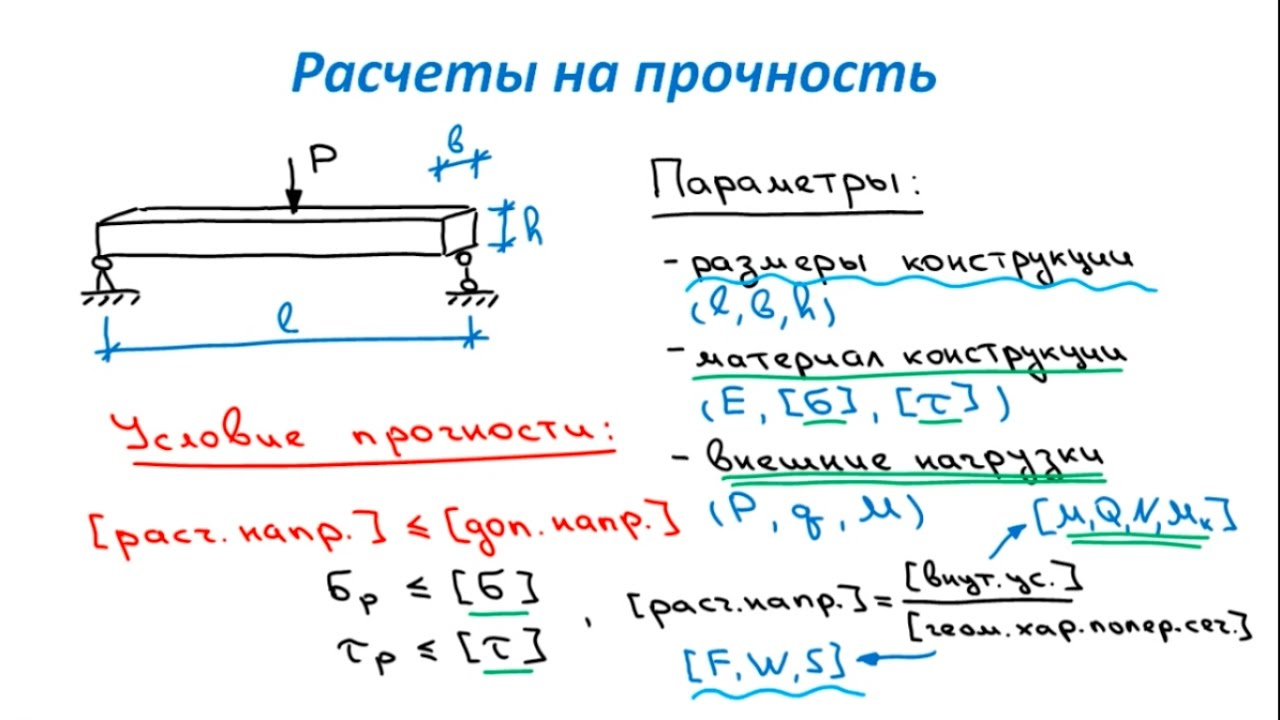
\includegraphics[height=6cm,width=1\textwidth,keepaspectratio]{basics_video.jpg}}
        \label{fig:basics_video.jpg}
    \end{figure}
\end{frame}

\begin{frame}[t]{CAE worflow}
\framesubtitle{}
    \vspace{-0.6cm}
    \begin{figure}[H]
        \centering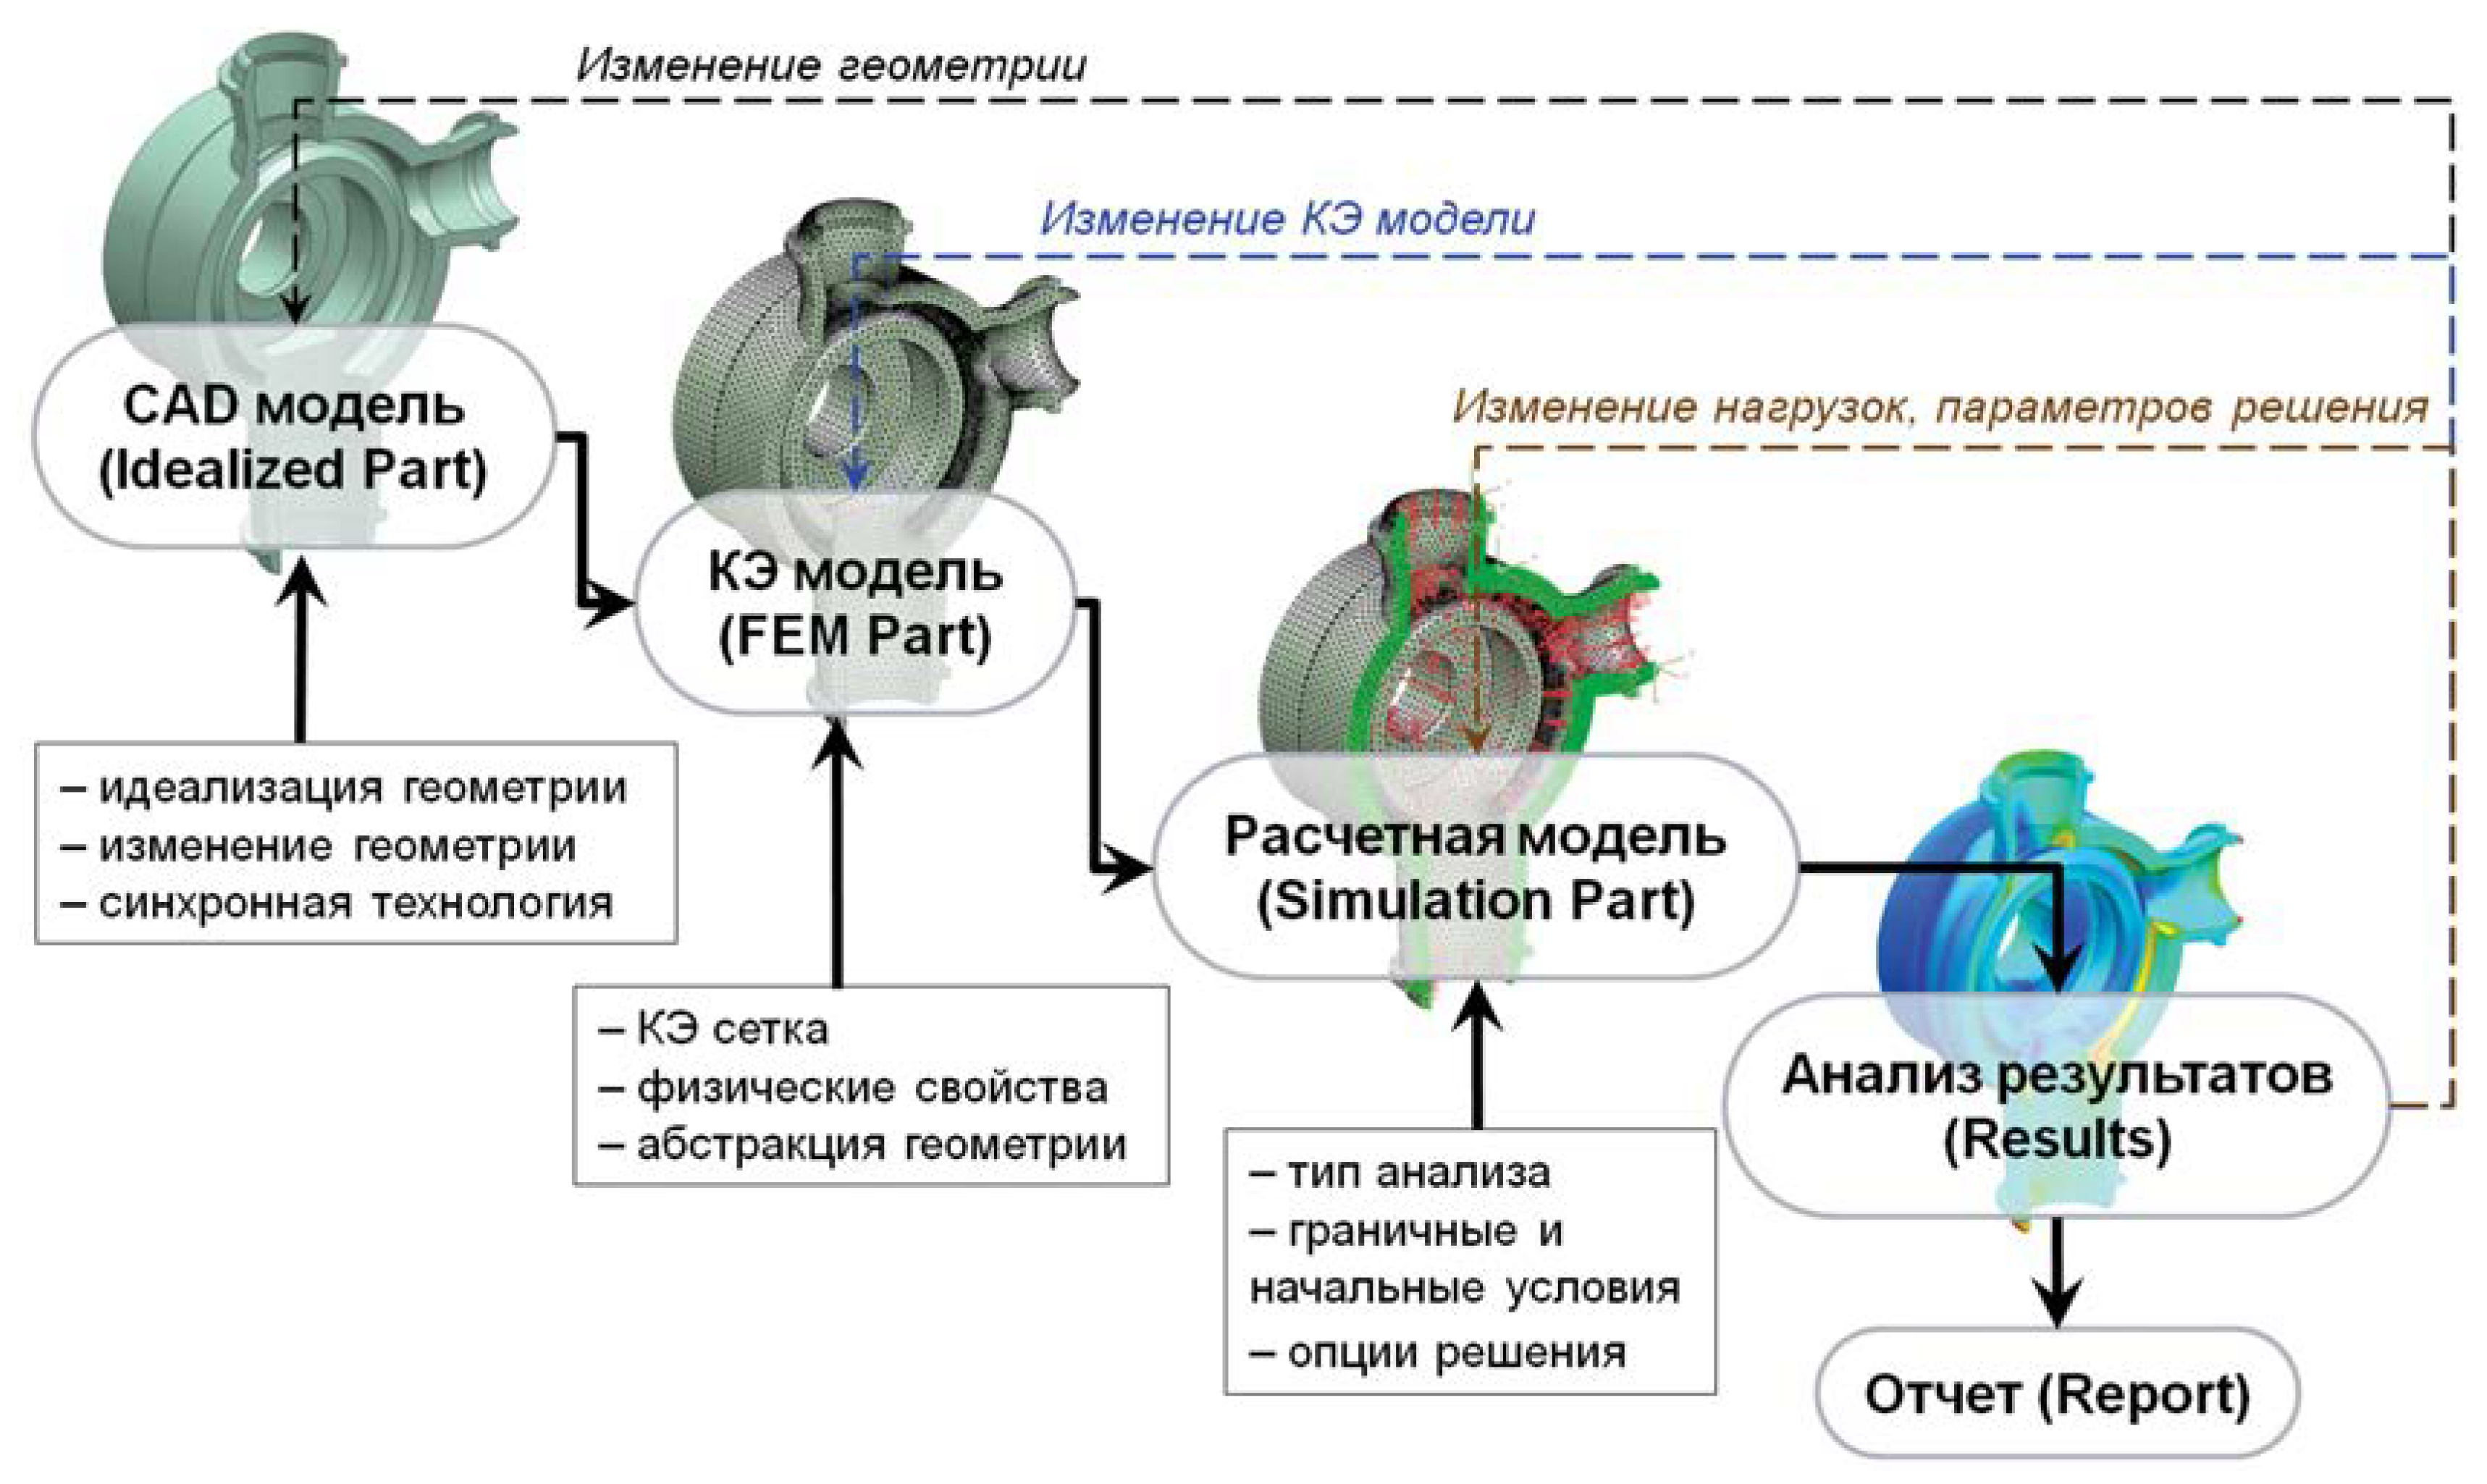
\includegraphics[height=6.5cm,width=1\textwidth,keepaspectratio]{cae_workflow.png}
        \label{fig:cae_workflow.png}
    \end{figure}
\end{frame}

\begin{frame}[t]{CAE designing scheme}
\framesubtitle{}
    \vspace{-0.6cm}
    \begin{figure}[H]
        \centering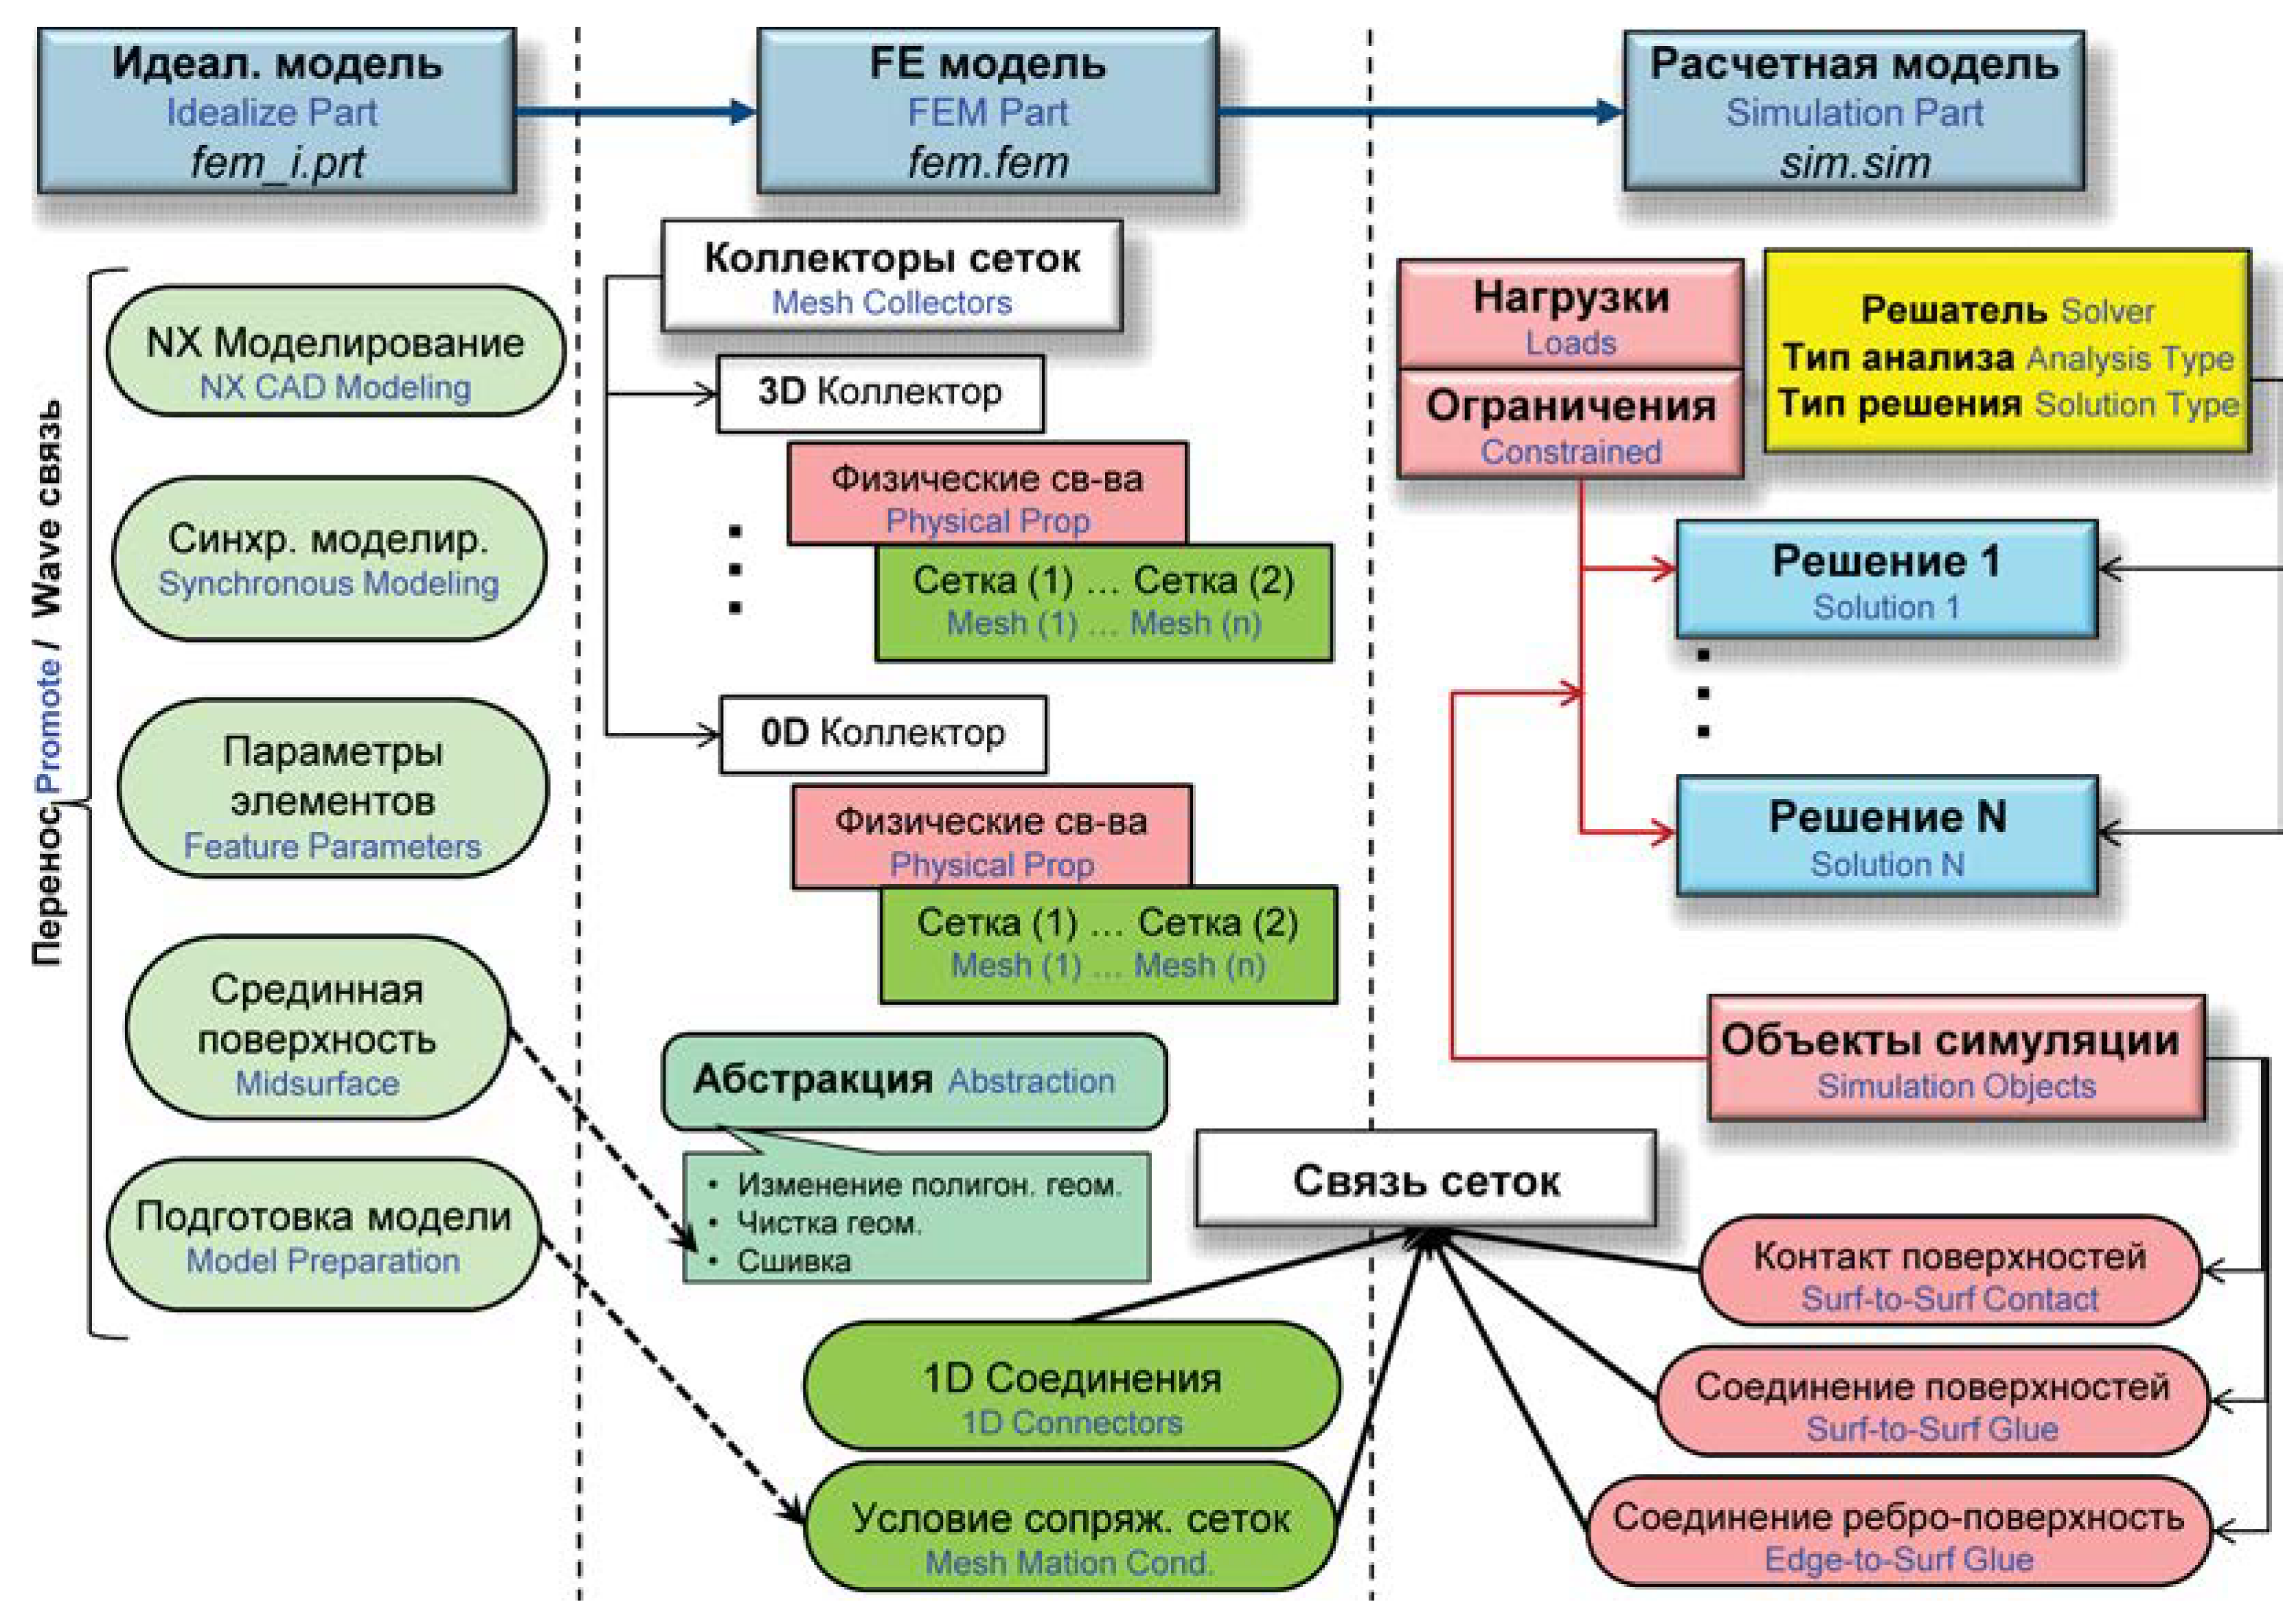
\includegraphics[height=6.5cm,width=1\textwidth,keepaspectratio]{cae_overview.png}
        \label{fig:cae_overview.png}
    \end{figure}
\end{frame}

\begin{frame}[t]{Types of Analysis in CAE}
    \framesubtitle{Video}
    \vspace{-0.6cm}
    \begin{figure}[H]
        \href{https://youtu.be/LyIHUFzO9kE}{
            \centering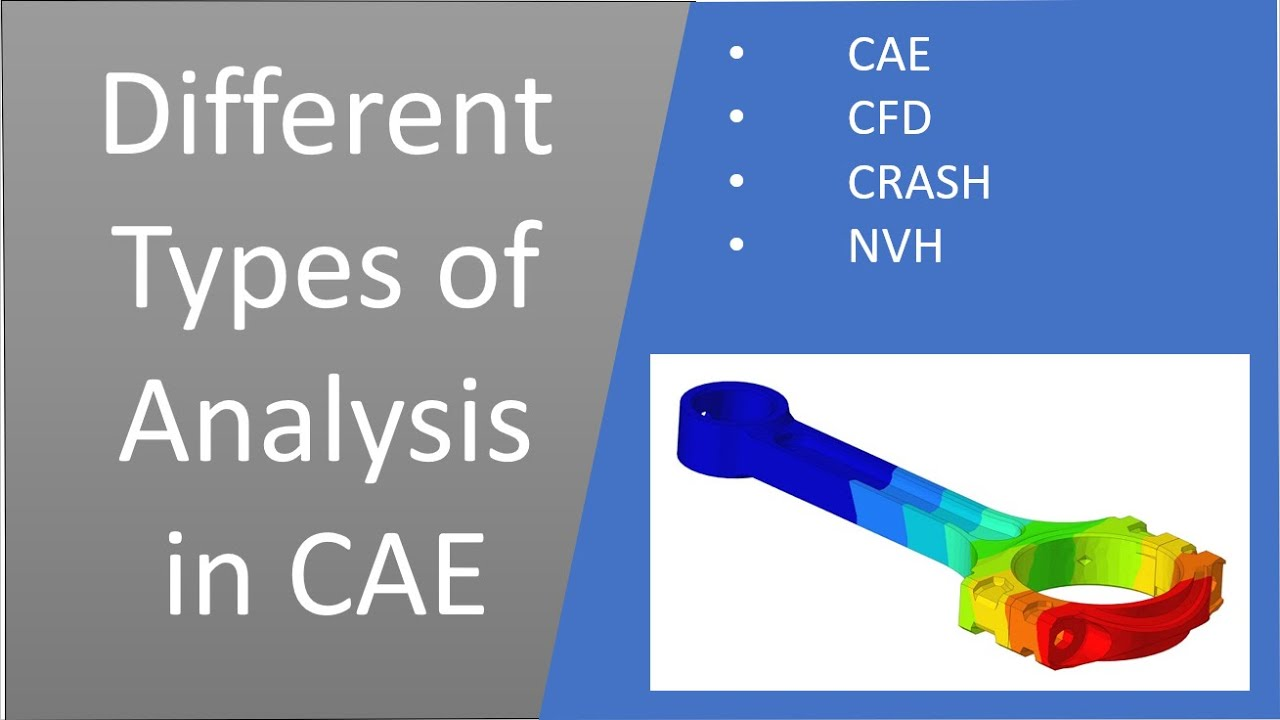
\includegraphics[height=6cm,width=1\textwidth,keepaspectratio]{types_of_analysis_in_cae_video.jpg}}
        \label{fig:types_of_analysis_in_cae_video.jpg}
    \end{figure}
\end{frame}

\begin{frame}[t]{Some real life case studies}
    \framesubtitle{Video}
    \vspace{-0.6cm}
    \begin{figure}[H]
        \href{https://youtu.be/BkTJ-PdliC4?t=374}{
            \centering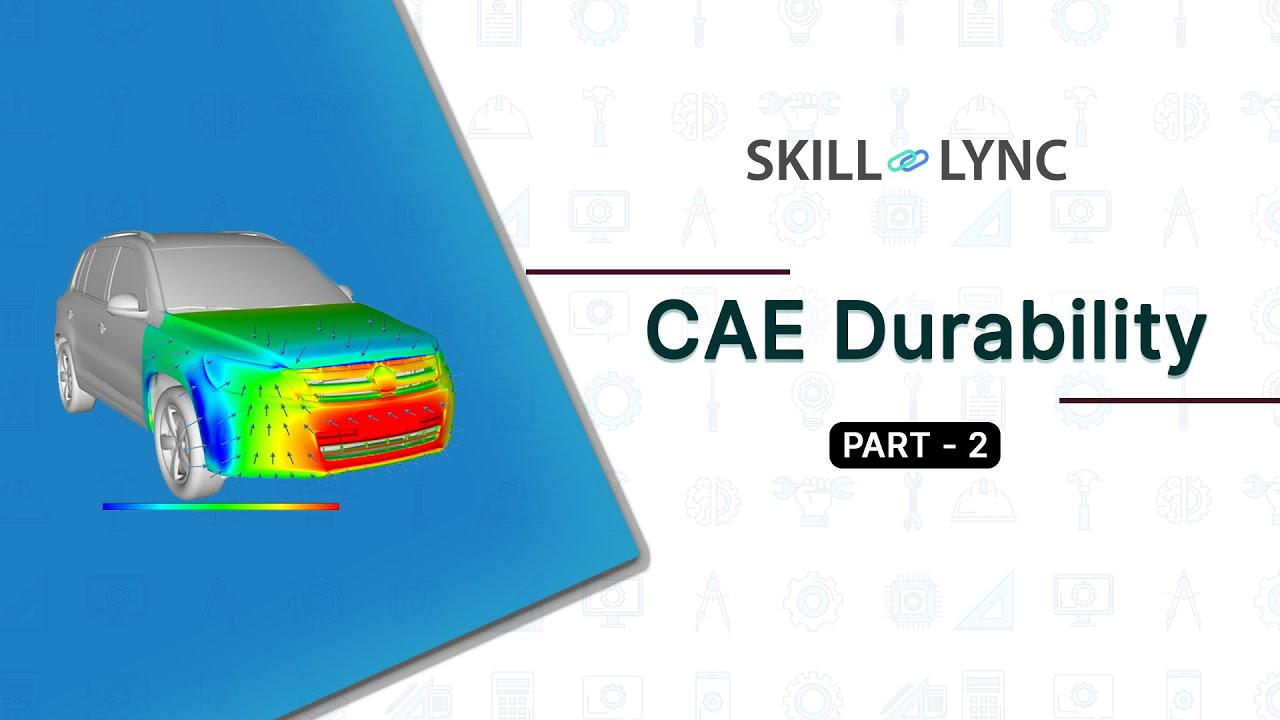
\includegraphics[height=6cm,width=1\textwidth,keepaspectratio]{cae_durability_video.jpg}}
        \label{fig:cae_durability_video.jpg}
    \end{figure}
\end{frame}

\begin{frame}[t]{Recomendations for creating meshes}
\framesubtitle{}
    \begin{itemize}
        \item Analyze beams, cables --- 1D mesh
        \item Sheet or shell component --- 2D mesh
        \item You should have more vertices in stress concentrator and large changes
        \item Try to eliminate chamfers, bendings, small holes
    \end{itemize}
\end{frame}

\begin{frame}[t]{First steps in CAE (Task 1, 2)}
    \framesubtitle{Video}
    \vspace{-0.6cm}
    \begin{figure}[H]
        \href{https://disk.yandex.ru/i/zj26vr7Uk03ilA}{
            \centering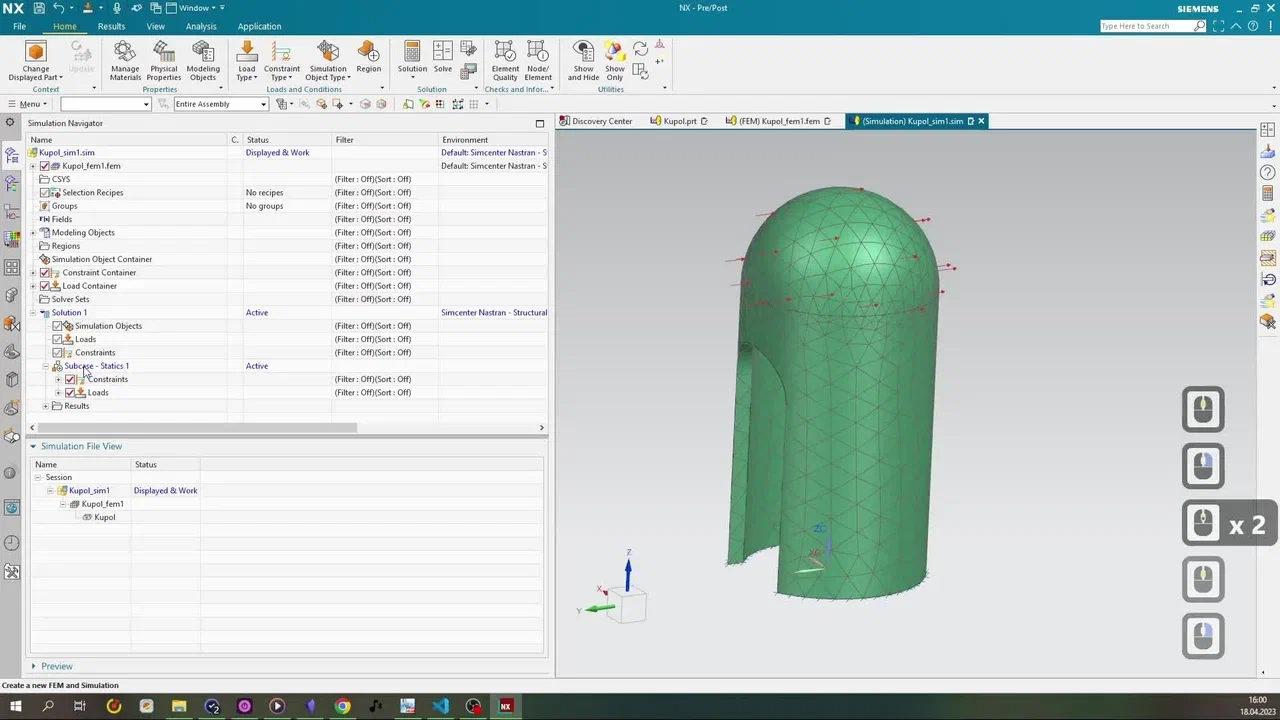
\includegraphics[height=6cm,width=1\textwidth,keepaspectratio]{basics_cae_video.png}}
        \label{fig:basics_cae_video.png}
    \end{figure}
\end{frame}

\begin{frame}[t]{2D mesh for sheet material + 1D for bolts (Task 1)}
    \framesubtitle{Video}
    \vspace{-0.6cm}
    \begin{figure}[H]
        \href{https://www.youtube.com/watch?v=3hZTIqXxq1o}{
            \centering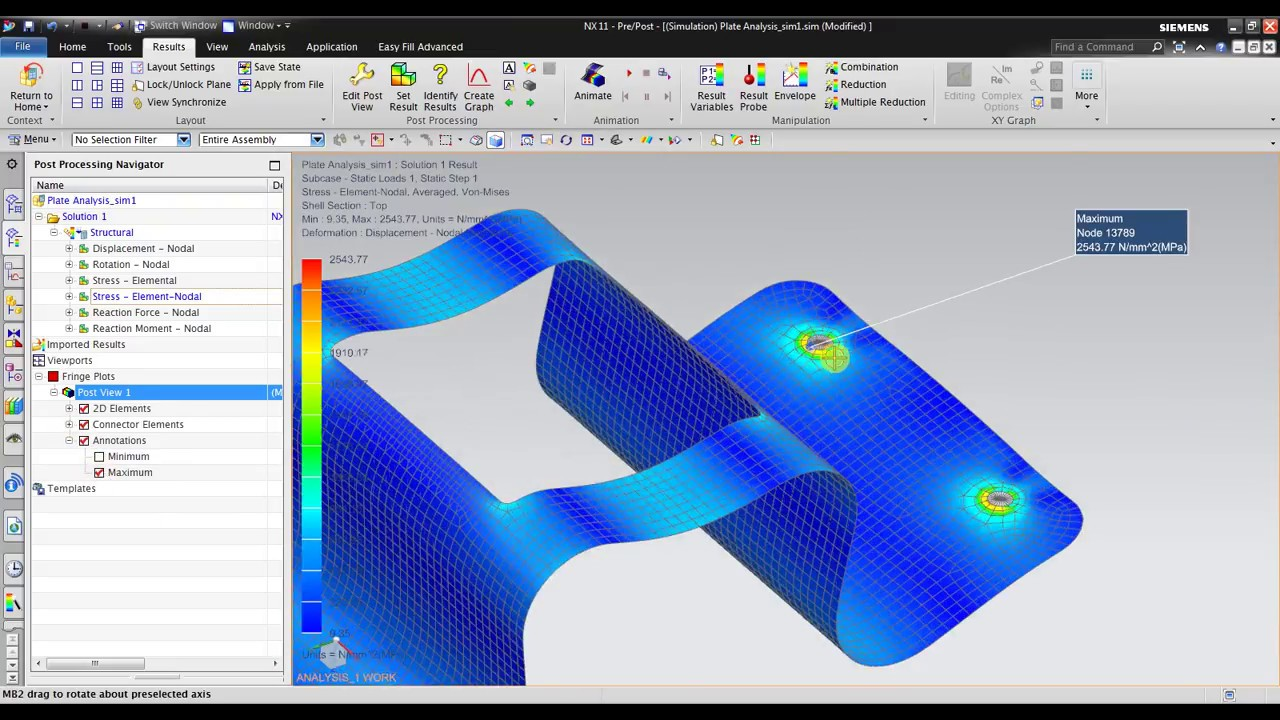
\includegraphics[height=6cm,width=1\textwidth,keepaspectratio]{two_d_sheet_video.jpg}}
        \label{fig:two_d_sheet_video.jpg}
    \end{figure}
\end{frame}

\begin{frame}[t]{Mesh Mating (optional)}
    \framesubtitle{Video}
    \vspace{-0.6cm}
    \begin{figure}[H]
        \href{https://youtu.be/mHD2vp394AI}{
            \centering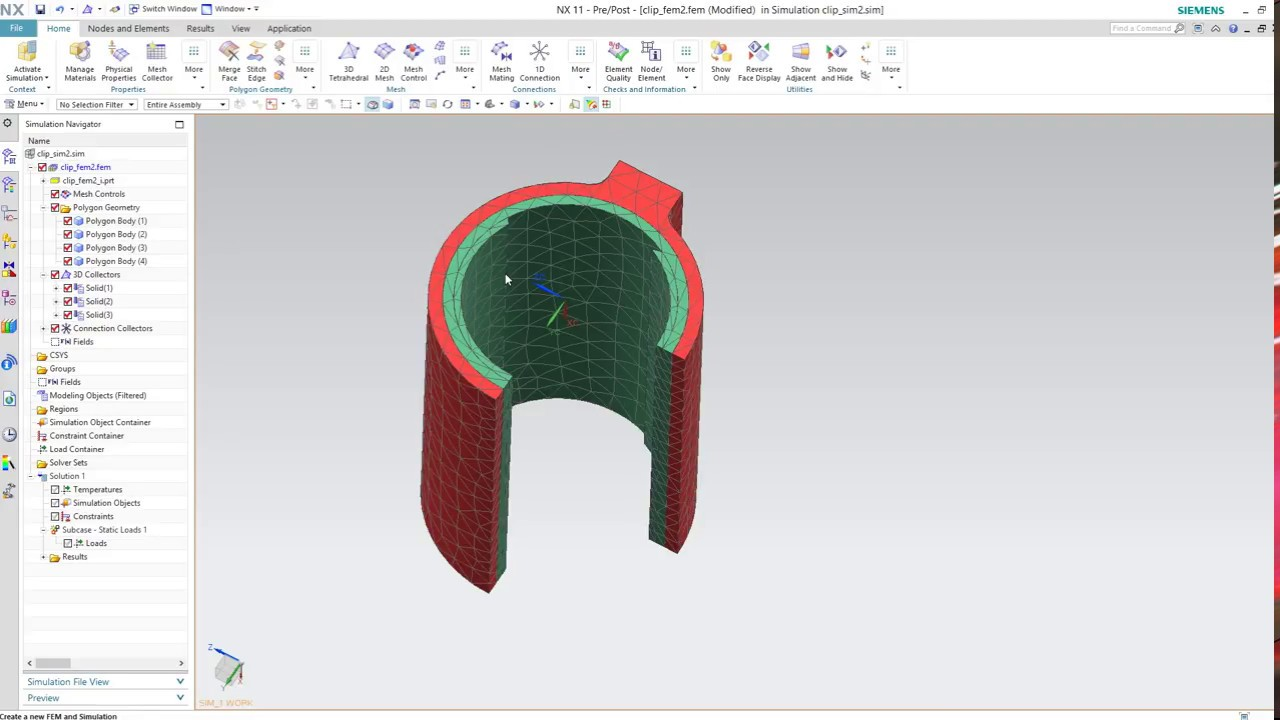
\includegraphics[height=6cm,width=1\textwidth,keepaspectratio]{mesh_mating_video.jpg}}
        \label{fig:mesh_mating_video.jpg}
    \end{figure}
\end{frame}

\begin{frame}[t]{Thermal simulation (Task 2)}
    \framesubtitle{Video}
    \vspace{-0.6cm}
    \begin{figure}[H]
        \href{https://youtu.be/mLqTBOaz9-w}{
            \centering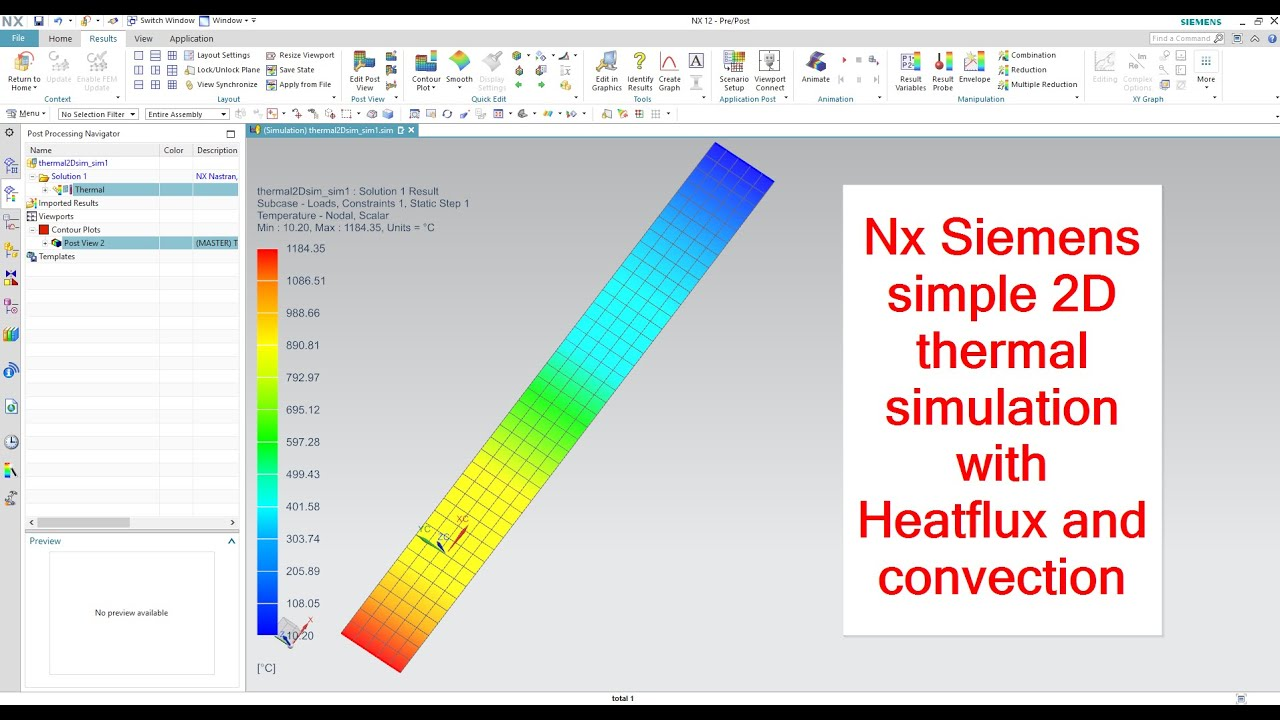
\includegraphics[height=6cm,width=1\textwidth,keepaspectratio]{thermal_sim_video.jpg}}
        \label{fig:thermal_sim_video.jpg}
    \end{figure}
\end{frame}

\begin{frame}[t]{Contact (Task 3)}
    \framesubtitle{Video}
    \vspace{-0.6cm}
    \begin{figure}[H]
        \href{https://youtu.be/2SoCy4tP74g}{
            \centering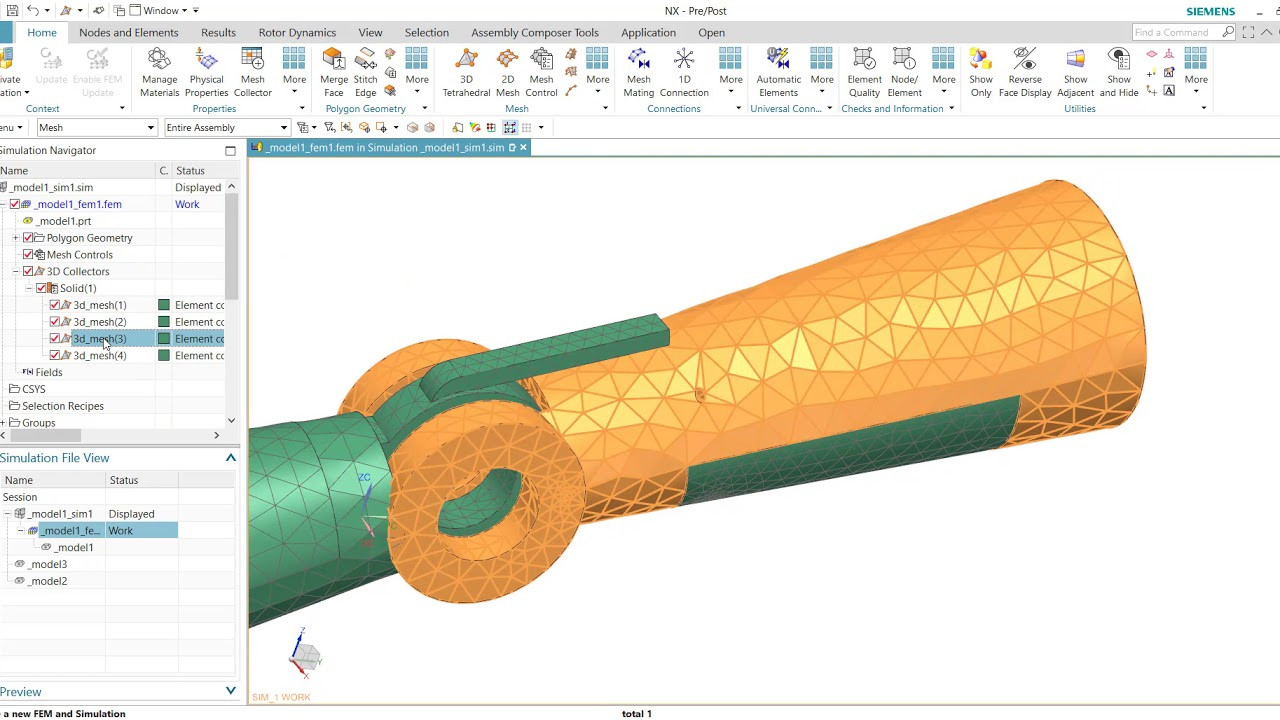
\includegraphics[height=6cm,width=1\textwidth,keepaspectratio]{good_case_study_video.jpg}}
        \label{fig:good_case_study_video.jpg}
    \end{figure}
\end{frame}

\begin{frame}[t]{Contact, Assembly (Task 3, 4)}
    \framesubtitle{Video}
    \vspace{-0.6cm}
    \begin{figure}[H]
        \href{https://disk.yandex.ru/i/yfhUfCk8MthoIw}{
            \centering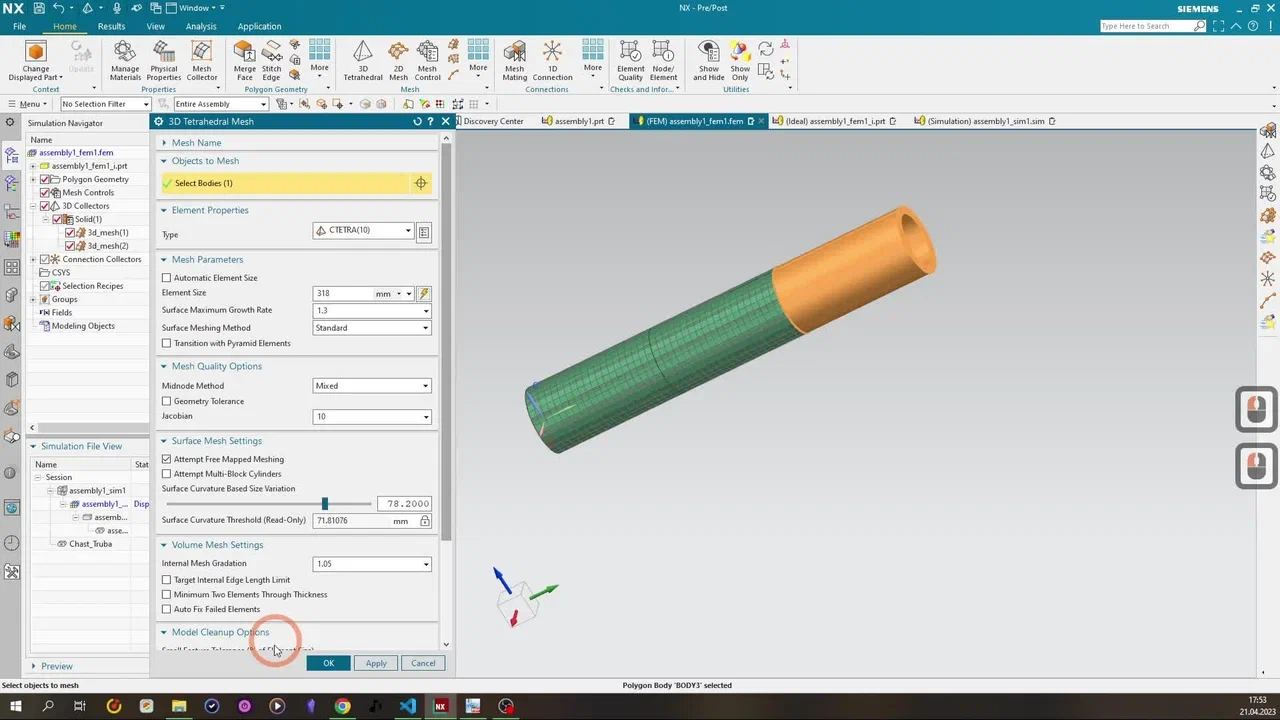
\includegraphics[height=6cm,width=1\textwidth,keepaspectratio]{cae_contact_assembly_video.png}}
        \label{fig:cae_contact_assembly_video.png}
    \end{figure}
\end{frame}

\begin{frame}[t]{Assembly Meshing (Multiple repeated parts) (Task 4)}
    \framesubtitle{Video}
    \vspace{-0.6cm}
    \begin{figure}[H]
        \href{https://youtu.be/PCvw1kOc5oE}{
            \centering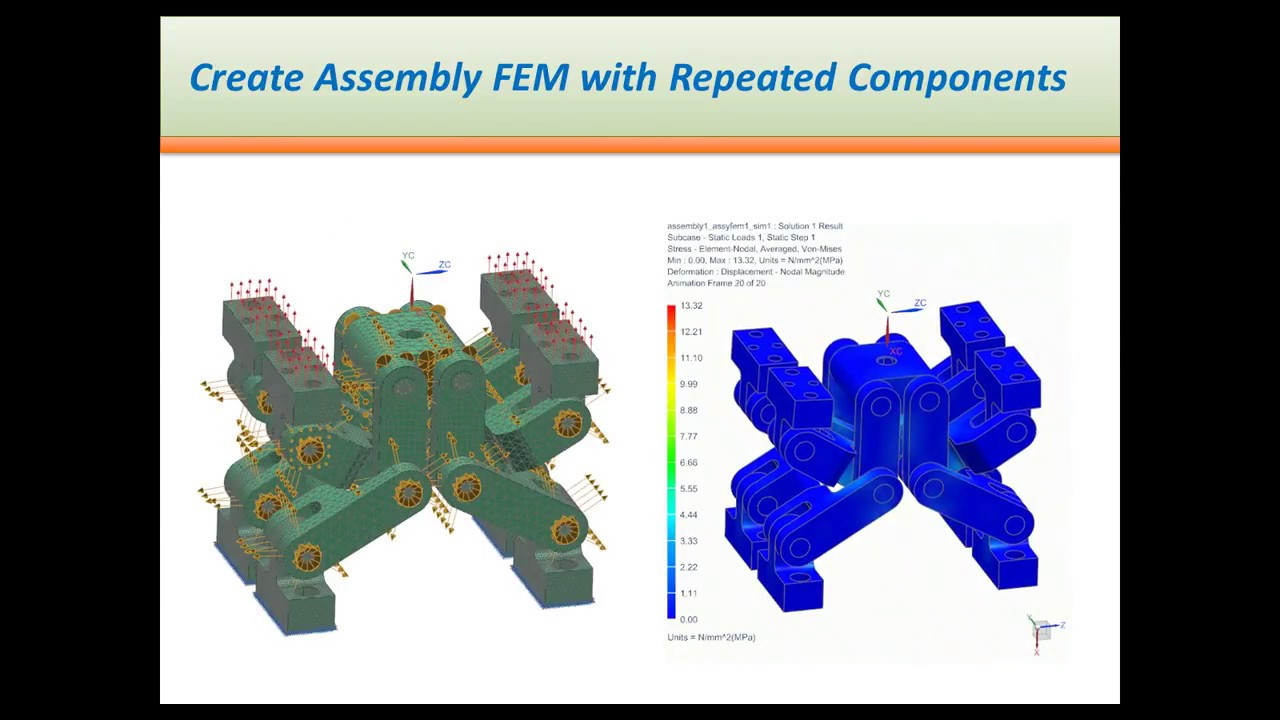
\includegraphics[height=6cm,width=1\textwidth,keepaspectratio]{assembly_meshing_video.jpg}}
        \label{fig:assembly_meshing_video.jpg}
    \end{figure}
\end{frame}

\begin{frame}[t]{Reference Material}
    \framesubtitle{}
    \begin{enumerate}
        \item \href{https://disk.yandex.ru/d/Q6H7la7iLdeh5Q}{Link to all needed books (IMPORTANT)}
        \item \href{https://youtu.be/vBilPNT2POM}{1D Bolt Simulation Double Plate Bolted Together}
        \item \href{https://youtu.be/xqBRiOuGGfw}{Introduction of Basic Simulation in NX CAE}
        \item \href{https://youtu.be/e0mKgo4m-kk}{How to add new material (rus)}
        \item \href{https://www.youtube.com/playlist?list=PLrlbZU2HDT4n-BPs-EW9x2PCWBDqmRi5H}{NX CAE. Основы расчетов на прочность в NX}
        \item \href{https://youtu.be/1jJtZCUNQNo}{CAE Durability, PART-1}
    \end{enumerate}
    \end{frame}

\fbckg{fibeamer/figs/last_page.png}
\frame[plain]{}

\end{document}